\chapter{Methods}

\section{System Overview and Architectural Design}

This section presents the architecture of the proposed workflow for AI-assisted building-footprint quality assessment and selective geometric refinement. The workflow is organized as a modular two-stage system that first evaluates existing building polygons against high-resolution aerial imagery and then applies segmentation-based refinement only where correction is considered useful. This design separates semantic assessment from geometric correction and allows the individual components of the pipeline to be inspected, adapted, and evaluated independently.

\begin{figure}[htbp]
\centering
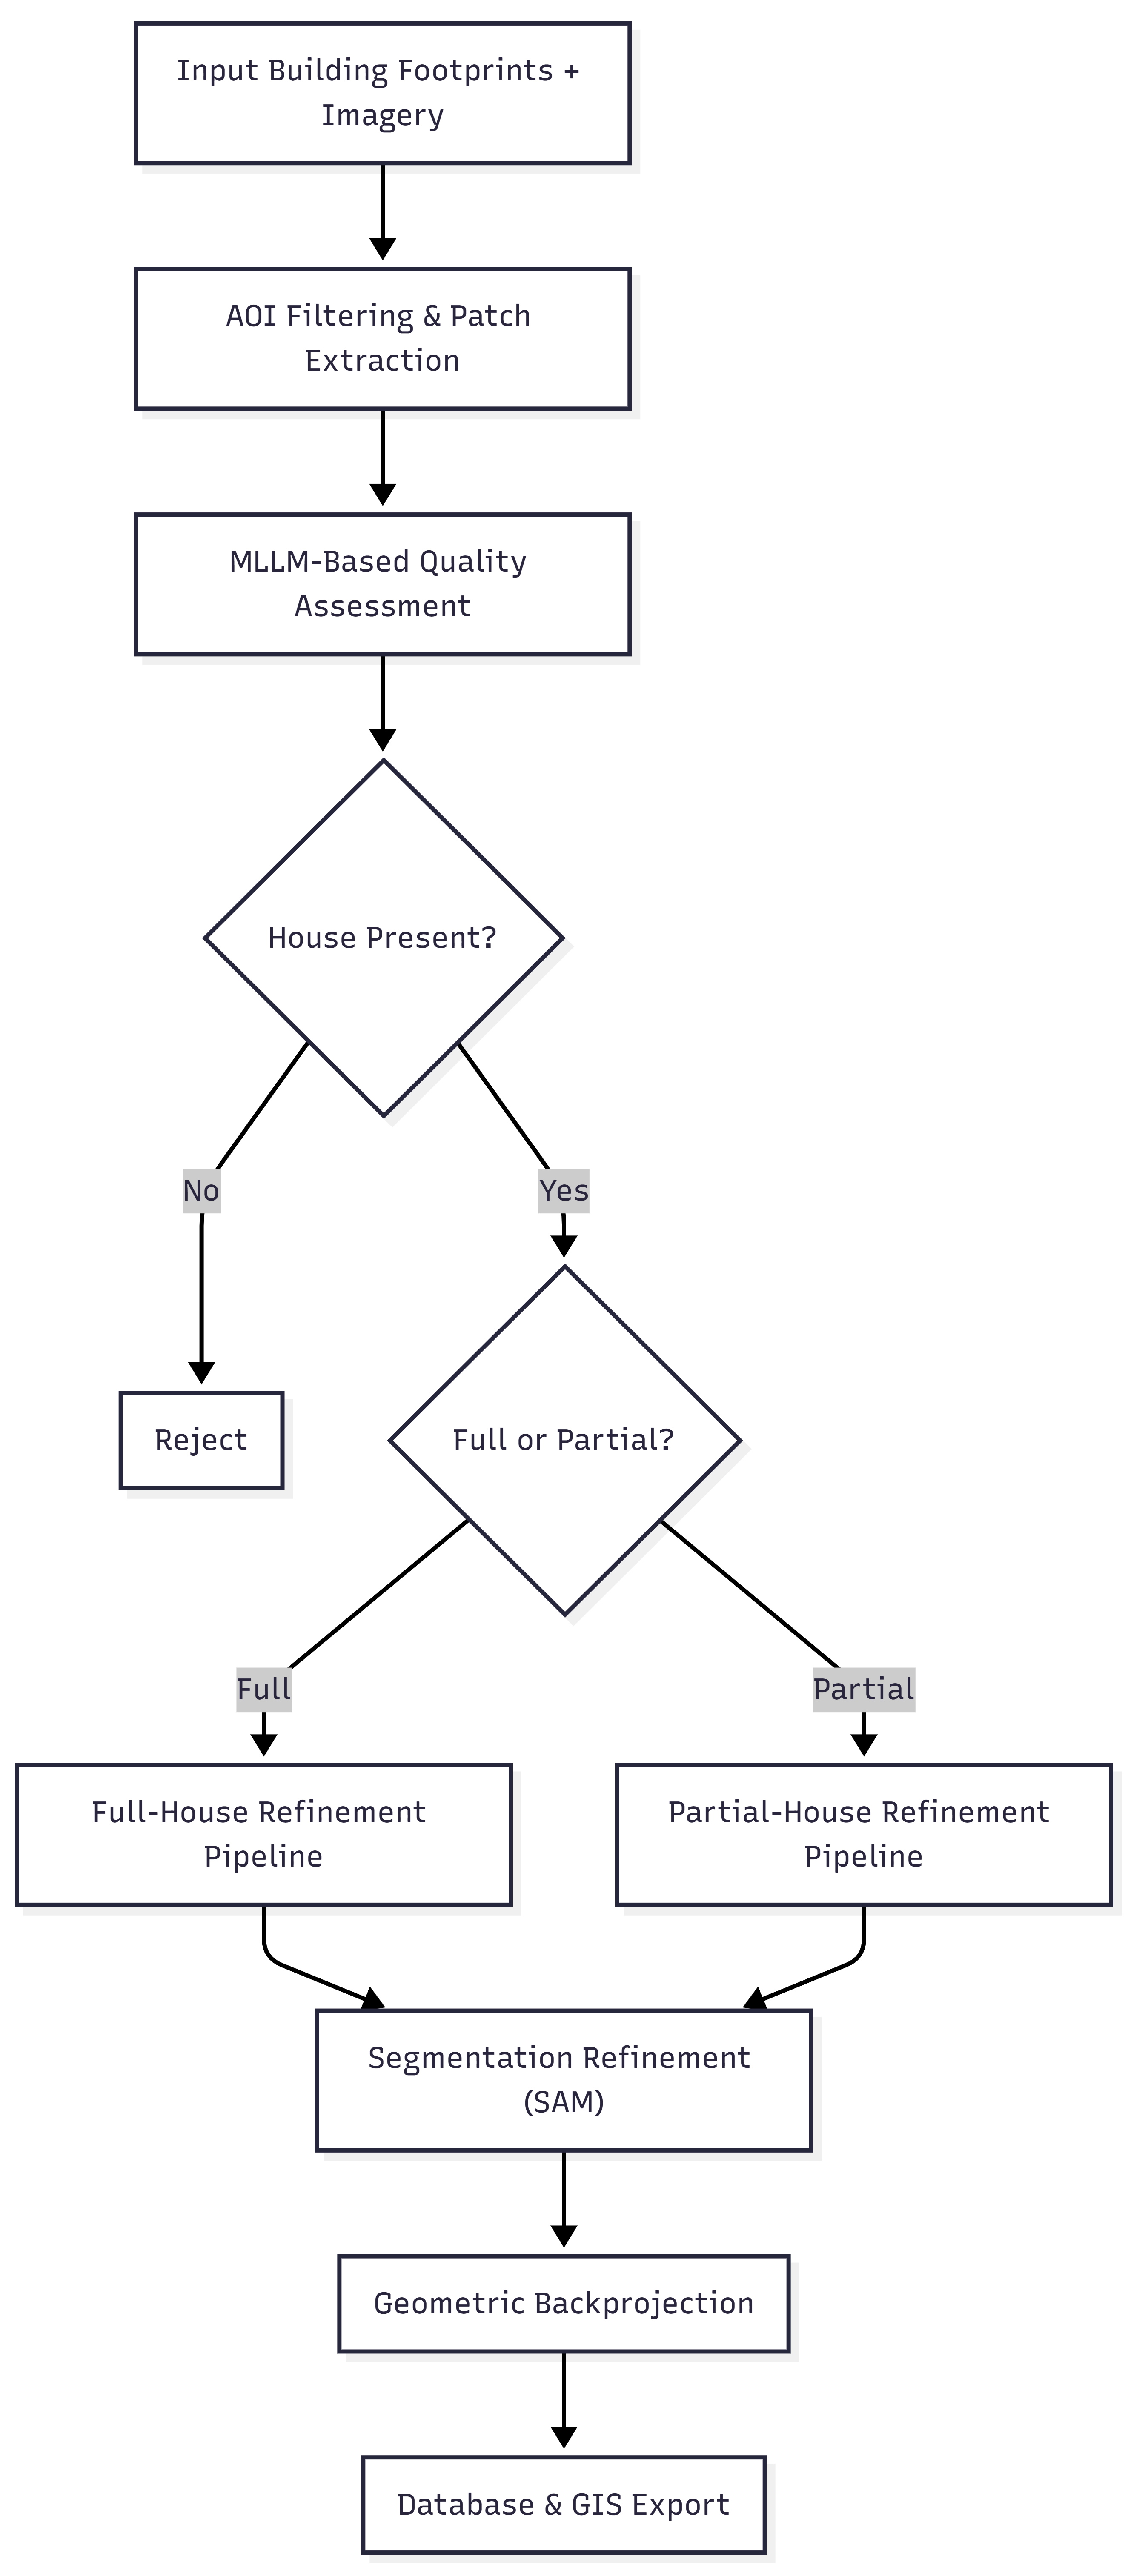
\includegraphics[scale=0.3]{Franzelin_Master/img/Flowchart_Main.png}
\caption{Overview of the proposed workflow for multimodal building footprint validation and refinement. Own illustration.}
\label{fig:workflow}
\end{figure}

The architecture follows a decoupled design in which evaluation, routing, prompt generation, segmentation, and geometric post-processing are implemented as separate but connected processing steps. This separation enables transparent decision-making, controlled refinement, and modular extensibility. The following subsections first introduce the conceptual motivation of the approach and then describe the end-to-end processing pipeline.

\subsection{Research Concept}

The focus of this work is to evaluate a new strategy for validating and improving large-scale geospatial datasets in settings where authoritative reference data are limited or unavailable. In this thesis, the approach is applied specifically to building footprints, with particular emphasis on the Google Open Buildings dataset. As discussed in Section~\ref{sec:QualityAssurance}, many existing quality-assessment strategies rely on comparisons with authoritative or independently validated reference datasets, as demonstrated in previous building-footprint quality-assessment workflows \citep{Hongchao_QualityAssesmentOSM, Brovelli_OSM_SpatialAccuracy, okyere2025evaluating}.

However, this reference-based paradigm is difficult to apply in regions where no high-quality ground truth dataset exists. This situation is particularly relevant in rural and peri-urban areas of the Global South, which form the main geographic focus of this work \citep{herfort2023spatio}. In such contexts, automatically generated datasets may be the only available source of building information, even though they can contain positional, completeness, and geometric errors. Consequently, alternative validation strategies are needed that can assess building-footprint quality directly from available imagery rather than from authoritative reference data.

The proposed solution is a two-stage framework that combines multimodal reasoning with segmentation-based geometry refinement. In the first stage, a multimodal large language model (MLLM) evaluates the relationship between an existing building polygon and the corresponding aerial image patch. The model is used to determine whether a visible roof structure is present, whether the polygon plausibly represents the visible building, and how the case should be routed within the workflow.

In the second stage, buildings identified as potentially improvable are processed with a SAM-based segmentation component. The segmentation model generates image-derived building-mask candidates, guided by spatial prompts produced during the MLLM stage. These candidates are subsequently regularized to improve their usability as GIS building footprints.

The core idea of the framework is therefore not to replace expert mapping or official validation standards, but to explore whether foundation models can support image-based quality assessment and candidate generation in data-scarce geospatial environments. The workflow is designed as a proof-of-concept for selective improvement: it aims to identify problematic footprints, generate plausible correction candidates, and provide a structured basis for potential human-in-the-loop validation.

\subsection{Overall Processing Pipeline}

The system architecture was implemented in Python and is connected to a PostgreSQL/PostGIS database for managing spatial data and storing intermediate and final processing results. The workflow, illustrated in Figure~\ref{fig:workflow} can be conceptually divided into seven main processing stages:

\textbf{1. Data Loading and AOI Filtering}

The workflow begins by loading building footprints from a spatial database. Only buildings intersecting a predefined Area of Interest (AOI) are selected for further processing. 

\textbf{2. Patch Extraction from Raster Imagery}

For each building footprint, an image patch is extracted from the corresponding aerial imagery. The patch contains the building and its surrounding context and serves as the common input representation for both the multimodal reasoning model and the segmentation model.

\textbf{3. MLLM-Based Quality Assessment}

The multimodal large language model evaluates the extracted patch to determine whether a building roof is present and whether the footprint plausibly captures the visible structure. This step provides a semantic interpretation of the building geometry that complements purely geometric validation methods.

\textbf{4. Routing into Refinement Pipelines}

Based on the assessment results, buildings are routed into different refinement pipelines. Buildings that appear complete are processed differently from those where only a partial structure is detected.

\textbf{5. Prompt Generation}

For buildings requiring refinement, spatial prompts are generated to guide the segmentation model. These prompts indicate regions belonging to the building and regions that should be excluded.

\textbf{6. Visual Model Refinement}

The segmentation model uses the generated prompts to produce an improved building mask that better aligns with the visible roof structure.

\textbf{7. Polygon Backprojection and Database Update}

Finally, the refined geometry is transformed back into geographic coordinates and stored in the spatial database together with additional metadata describing the refinement process.


\section{Data Sources and Preprocessing}

\subsection{Building Footprint Datasets}

This study uses automatically generated building footprint datasets derived from large-scale remote sensing data. The primary dataset considered in this work is the Google Open Buildings dataset, which provides building footprints across large parts of the Global South, including Africa, Latin America, and parts of South and Southeast Asia. The dataset was generated using deep learning methods applied to high-resolution satellite imagery with a spatial resolution of approximately 50\,cm per pixel \citep{sirko2021continentalscalebuildingdetectionhigh, googleopenbuildings}.

The underlying detection pipeline is based on a convolutional neural network architecture derived from U-Net, which performs semantic segmentation to classify each pixel in an image as either building or non-building. Detected building regions are subsequently converted into polygon footprints through connected-component analysis and vectorization. The model was trained on approximately 100,000 manually annotated satellite image tiles containing around 1.75 million labeled building instances. After training and large-scale inference across the African continent, the resulting dataset contains approximately 516 million detected building footprints \citep{sirko2021continentalscalebuildingdetectionhigh}.

The Open Buildings dataset has a continent-scale coverage and includes a wide variety of settlement types, from dense urban environments to small rural buildings. Due to this large geographic diversity, the dataset captures many different building styles, roof materials, and settlement patterns. However, the automatic generation process also introduces characteristic errors, including incomplete footprints, merged buildings in dense settlements, and geometric simplifications, as discussed in Section~\ref{sec:building_errors}.

In this thesis, only small subsets of the dataset are used rather than processing the complete global dataset. The selected areas are chosen based on the availability of high-resolution aerial imagery that spatially overlaps with the building footprints (see Chapter~\ref{ch:study_area}). This ensures that each building polygon can be visually compared against the underlying imagery, which is required for the multimodal quality assessment and refinement workflow proposed in this study.


\subsection{Imagery Data}

High-resolution aerial or satellite imagery is used as the visual reference for evaluating and refining building footprints. These images provide the visual context required by both the multimodal reasoning model and the segmentation model. In this study, imagery is primarily obtained from the open imagery platform OpenAerialMap (OAM). OAM is a crowdsourcing platform that enables users to upload, host, and share openly licensed aerial imagery collected from drones, aircraft, or satellites. The platform was originally developed to support rapid mapping during humanitarian crises and disaster response scenarios, but it has since evolved into a widely used repository for openly accessible aerial imagery \citep{openaerialmap, MandourahHochmair2024}.

For the purposes of this study, OpenAerialMap provides a convenient and scalable imagery source that allows access to high-quality aerial imagery without requiring complex data acquisition workflows. Since the geographic location of the imagery is not a critical factor for the methodological evaluation performed in this thesis, the platform offers a practical way to obtain diverse high-resolution imagery suitable for testing and evaluating the proposed quality assessment and refinement pipeline.

\subsection{Patch Generation and Rendering}

For each selected building footprint, a square image patch is extracted from the corresponding GeoTIFF raster. The building geometry is first transformed from its original vector coordinate reference system (CRS) into the raster CRS. A square window is then constructed around the centroid of the footprint. The window size is determined by the maximum spatial extent of the building multiplied by a configurable \emph{context factor} (see Appendix \ref{app:core_parameters}), ensuring that sufficient surrounding visual information is captured.

The raster window is read and resized to a standardized resolution of $512 \times 512$ pixels. Standardizing the patch size ensures consistent input dimensions for both the multimodal large language model (MLLM) and the segmentation model.

Simultaneously, the building geometry is transformed into the coordinate system of the extracted patch through the following transformation chain:

\begin{equation}
\begin{aligned}
\text{Vector CRS}
&\longrightarrow \text{Raster CRS}
\longrightarrow \text{window pixel space} \\
&\longrightarrow 512 \times 512\ \text{patch space}.
\end{aligned}
\end{equation}

To support different stages of the workflow, three different patch representations are generated. 
Each representation contains only the information required for the corresponding processing step. 
Providing unnecessary visual elements could introduce noise and potentially confuse the multimodal large language model (MLLM) or the segmentation model. 
Therefore, separate patch variants are created for the same building in order to include only the relevant visual cues needed for each stage of the pipeline.


\begin{itemize}
    \item \texttt{Segmentation patch:} Plain RGB image without overlays, used as input for segmentation.
    \item \texttt{Assessment patch:} Image with the original building polygon overlaid, used for MLLM-based semantic reasoning to determine whether a visible building is present beneath the polygon and whether the footprint should be routed to the full- or partial-building refinement pipeline.
    \item \texttt{Prompt-reference patch:} Image with a centered reference marker indicating the footprint centroid, used for structured prompt generation.
\end{itemize}

\begin{figure}[htb]
\centering

\begin{subfigure}{0.32\textwidth}
    \centering
    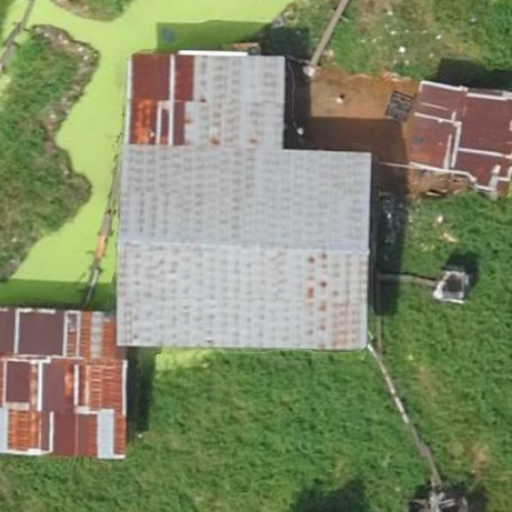
\includegraphics[width=\linewidth]{img/bld_1157971_raw.png}
    \caption{Segmentation patch}
\end{subfigure}
\hfill
\begin{subfigure}{0.32\textwidth}
    \centering
    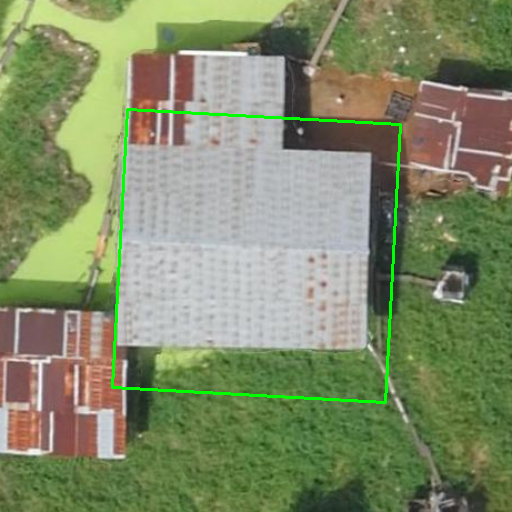
\includegraphics[width=\linewidth]{img/bld_1157971_clean.png}
    \caption{Assessment patch}
\end{subfigure}
\hfill
\begin{subfigure}{0.32\textwidth}
    \centering
    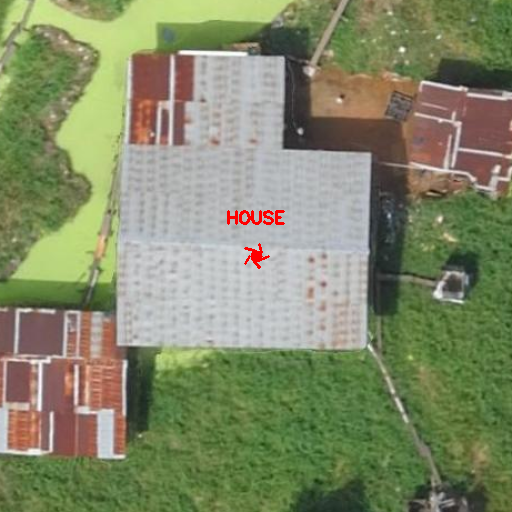
\includegraphics[width=\linewidth]{img/bld_1157971_debug.png}
    \caption{Prompt-reference patch}
\end{subfigure}

\caption{Example patch representations generated during preprocessing. The segmentation patch contains the original RGB imagery used for segmentation, the assessment patch overlays the original building footprint used for MLLM reasoning, and the prompt-reference patch includes a centroid reference marker used during prompt generation. All patches are normalized to a resolution of $512 \times 512$ pixels. Own illustration.}\label{fig:patch_types}

\end{figure}


During the refinement stage, patches may be re-extracted with an increased context factor to prevent boundary truncation effects. In the partial-house pipeline, additional localized sub-cropping is performed to isolate candidate building structures.


\section{MLLM-Based Quality Assessment}

\subsection{Model Configuration}

The MLLM-based quality assessment was performed using Qwen3-VL-8B-Instruct served through a vLLM backend on a remote GPU instance. Each request consisted of one image patch and a task-specific text prompt. Image inputs were provided at a standardized resolution of \(512 \times 512\) pixels. The model outputs were requested in a structured format and parsed into predefined fields used for routing, semantic error description, and prompt generation. Invalid or unparsable outputs were stored as failed outputs and excluded from downstream analyses where necessary.

\subsection{Structured QA Framework}

In the third stage of the workflow, a multimodal large language model (MLLM) is used to perform semantic quality assessment of the extracted building patch. The MLLM receives the assessment patch representation (image with polygon overlay) and produces a structured, machine-readable evaluation.

The assessment consists of three core reasoning tasks.

Because this stage determines the downstream routing and refinement strategy, the MLLM-based assessment was implemented as a sequence of task-specific prompts rather than as a single combined instruction. Each prompt addresses one clearly defined reasoning step and returns a structured JSON field that can be parsed automatically by the pipeline \citep{Zaid_prompt_decompisiton}. The full prompt content and JSON schema are documented in Appendix~\ref{app:mllm_prompts} and Appendix~\ref{app:mllm_json_schema}. Table~\ref{tab:mllm_reasoning_tasks} summarizes the main reasoning tasks used for semantic quality assessment.


\begin{table}[htb]
\centering
\small
\caption{MLLM reasoning tasks used for semantic quality assessment and routing. The prompt objectives are summarized from the operational prompts documented in Appendix~\ref{app:mllm_prompts}.}
\label{tab:mllm_reasoning_tasks}
\begin{tabular}{p{0.23\linewidth}p{0.46\linewidth}p{0.21\linewidth}}
\toprule
\textbf{Reasoning task} & \textbf{Prompt objective} & \textbf{Parsed output} \\
\midrule

Building presence &
Determine whether a visually identifiable roof or man-made building structure is present inside the overlaid polygon. &
\texttt{house\_present} \\

Footprint coverage &
Evaluate whether the polygon captures the majority of the visible roof or only a partial section of the building. &
\texttt{full\_house\_present} \\

Geometric error analysis &
Assess spatial misalignment and identify semantic geometry errors such as \texttt{SHAPE\_MISMATCH}, \texttt{MISSING\_PARTS}, and \texttt{EXTRA\_PARTS}. &
\texttt{error\_tags}, \texttt{error\_description} \\

\bottomrule
\end{tabular}
\end{table}

First, the model determines whether a visually identifiable roof structure is present within the polygon boundary. If no building structure is detected, the footprint is excluded from further processing and only the quality assessment result is stored. This prevents unnecessary refinement of non-building objects or false positives.

Second, the MLLM evaluates whether the polygon captures the majority of the visible building structure. This distinction is critical for downstream processing. If the polygon contains most of the building extent, refinement can be performed relative to the existing footprint. However, if the polygon captures only a small portion of the building, the initial bounding box derived from the footprint may be too restrictive. In such cases, a discovery-oriented refinement strategy must be applied to identify the full building extent prior to geometric correction.

Third, the model generates a semantic error assessment using a separate error-analysis prompt chain. The first prompt evaluates whether the polygon is spatially misaligned, the second prompt assigns predefined geometric error tags such as \texttt{SHAPE\_MISMATCH}, \texttt{MISSING\_PARTS}, and \texttt{EXTRA\_PARTS}, and the final prompt returns a short JSON field containing a human-readable error description. The resulting tags and description are stored with the MLLM decision output.

The MLLM tasks were intentionally split into smaller prompt chains instead of being handled in one combined instruction. This design follows the idea of task decomposition, where complex reasoning tasks are broken down into simpler subproblems that can be answered sequentially \citep{zhou2022least}. A similar strategy has also been shown to improve reliability in zero-shot visual question-answering by separating a complex visual task into individual sub-prompts \citep{Zaid_prompt_decompisiton}.

The result of this stage is a decision object containing four key attributes:

\begin{itemize}
    \item \texttt{house\_present}: Boolean indicator of building presence.
    \item \texttt{full\_house\_present}: Boolean or null indicator distinguishing full versus partial building coverage.
    \item \texttt{error\_description}: Structured semantic explanation of detected inconsistencies.
    \item \texttt{error\_tags}: List of predefined semantic geometry error categories assigned by the MLLM, such as \texttt{SHIFTED}, \texttt{SHAPE\_MISMATCH}, \texttt{MISSING\_PARTS}, \texttt{EXTRA\_PARTS}, or \texttt{OVERSIMPLIFIED}.
\end{itemize}

\subsection{Decision Logic and Routing}
\label{sec:decision_logic_routing}

Based on the decision object generated by the MLLM, buildings are routed into different refinement pipelines.

\begin{table}[htb]
\centering
\caption{Deterministic routing rules derived from the structured MLLM decision object.}
\label{tab:routing_rules}
\begin{tabular}{ccc}
\toprule
\texttt{house\_present} & \texttt{full\_house\_present} & \textbf{Pipeline} \\
\midrule
False & -- & None \\
True & True & FullHousePipeline \\
True & False / Null & PartialHousePipeline \\
\bottomrule
\end{tabular}
\end{table}

If the building is classified as partial or uncertain, a discovery-oriented refinement strategy is applied before geometric correction.

Figure~\ref{fig:partial_pipeline} illustrates this situation. In some cases the original footprint only covers a subset of the visible building structure. If the building were directly processed by the standard refinement pipeline, the prompts and bounding boxes provided to the segmentation model would restrict the segmentation to this limited region. As a result, the segmentation model would only refine the already detected subsection of the building instead of reconstructing the full structure.

To avoid this limitation, the system expands the spatial context around the building before applying the discovery-oriented refinement step. While the standard assessment and full-house refinement patches are generated with a context factor of 1.5, partial-house cases are re-extracted with a larger context factor of 4.0 (see Appendix \ref{app:core_parameters}). This enlarged window allows the discovery step to search beyond the limited original footprint extent and to identify additional visible building parts before the final SAM-based refinement is performed.

\begin{figure}[htbp]
\centering

\begin{subfigure}{0.45\textwidth}
    \centering
    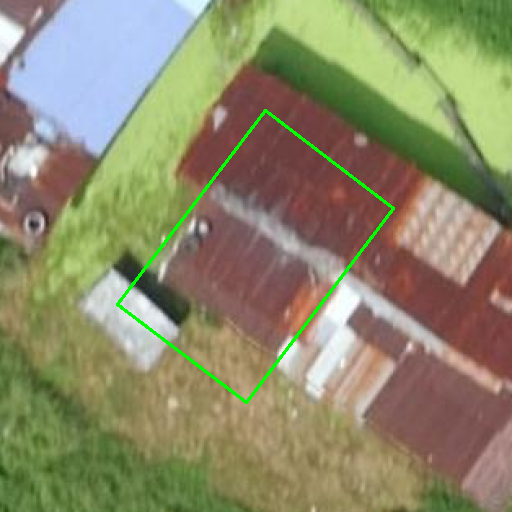
\includegraphics[width=\linewidth]{img/bld_1683655_clean.png}
    \caption{Initial footprint covering only part of the building}
\end{subfigure}
\hfill
\begin{subfigure}{0.45\textwidth}
    \centering
    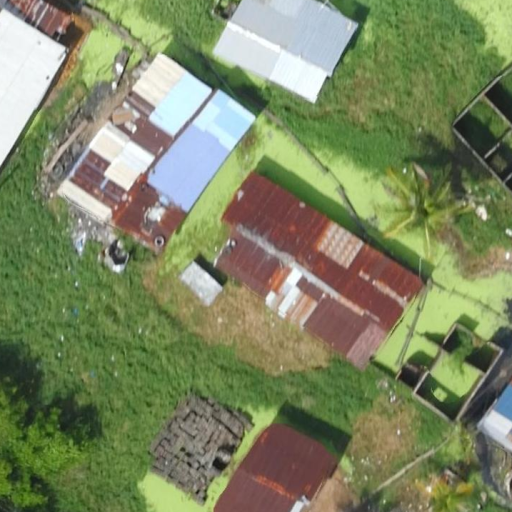
\includegraphics[width=\linewidth]{img/bld_1683655_partial_context.png}
    \caption{Expanded context used for structure discovery}
\end{subfigure}

\caption{Example of a partial building detection requiring context expansion. Own illustration.}
\label{fig:partial_pipeline}

\end{figure}

\section{Prompt Generation for the Visual Model}

Once a building has been routed into a refinement pipeline, spatial prompts must be generated to guide the segmentation model. Segment Anything (SAM) supports interactive prompting through a combination of positive points, negative points, and bounding boxes \citep{kirillov2023segment}.

In the proposed framework, prompt generation is performed automatically using the multimodal large language model (MLLM). The model receives the \emph{prompt-reference patch}, which contains the aerial image together with a visual reference marker indicating the centroid of the target building.

The prompt generation procedure produces two types of spatial constraints:

\begin{itemize}
\item \textbf{Positive points (inside points)} that lie on the roof surface of the target building.
\item \textbf{Negative points (outside points)} that lie outside the building.
\end{itemize}

The MLLM operates in a normalized coordinate system ranging from $(0,0)$ in the upper left corner to $(1000,1000)$ in the lower right corner of the image. The generated coordinates are then transformed into the pixel coordinate system of the patch.

Positive points are generated sequentially to ensure spatial coverage across the roof surface, while negative points help distinguish the building from surrounding structures.

In addition to point prompts, a bounding box derived from the original footprint geometry is used to constrain the search region of the segmentation model.

The resulting prompt configuration consists of:

\begin{itemize}
\item three positive roof points,
\item three negative background points,
\item one bounding box derived from the original footprint.
\end{itemize}

\section{Segmentation-Based Footprint Refinement}
\begin{wrapfigure}[40]{r}{0.45\textwidth}
\centering
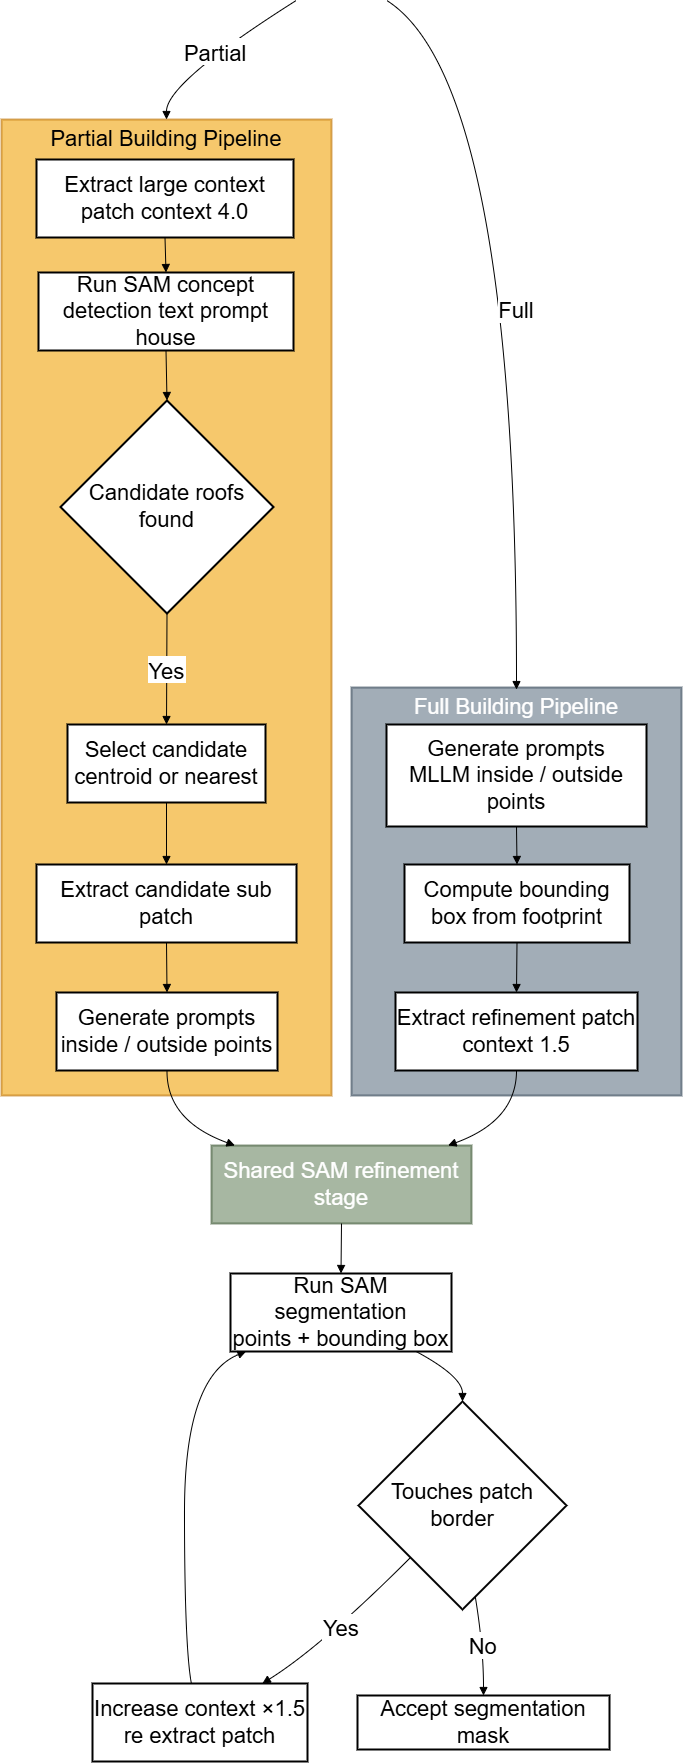
\includegraphics[width=\linewidth]{Franzelin_Master/img/Flowchart_SAMStage.drawio.png}
\caption{Visual model refinement workflow. Own illustration.}
\label{fig:sam_stage}
\end{wrapfigure}
After the prompt generation stage, the building refinement process is performed using a visual segmentation foundation model. While the MLLM provides semantic interpretation and spatial guidance, the visual model is responsible for producing a geometrically precise building mask based on the underlying imagery.

The refinement stage consists of four main components:

\begin{itemize}
\item segmentation using text prompt,
\item segmentation using visual prompts,
\item iterative refinement and context expansion,
\item conversion of segmentation masks into geospatial vector geometries.
\end{itemize}

For the geometric refinement stage, the Segment Anything model family was used as the visual segmentation backbone \citep{kirillov2023segment, papersam3}. The final backend used in the implementation is specified below.

\subsection{Segmentation Model and Prompting Interfaces}

In this thesis, the term SAM-based refinement refers to the visual segmentation component used for prompt-based building-mask generation. The final implementation used a local SAM 3 checkpoint (\texttt{sam3.pt}) as the segmentation backend. Point- and box-guided refinement used the visual-prompt interface, while the text-prompted discovery step in the \textit{PartialHousePipeline} used the SAM 3 concept-prompted backend. 

In this work, the pretrained SAM-based backend was used without further architectural modifications. Preliminary experiments were conducted to fine-tune a previous model version (SAM 2) using building footprint data derived from two datasets: the Inria Aerial Image Labeling dataset and the SpaceNet 2 dataset for the Khartoum area. Approximately 1000 training patches were generated from these datasets. The two datasets represent different architectural contexts: the Inria dataset predominantly contains buildings from Western urban environments with pitched or heterogeneous roof structures, whereas the Khartoum dataset primarily consists of flat concrete roofs typical for dense settlements in Sudan.

Despite these experiments, the fine-tuned model did not improve segmentation performance. Instead, it showed clear signs of overfitting to specific roof textures and building patterns present in the training data. In particular, the model tended to over-segment roofs and to introduce artificial boundaries within single buildings, especially when roof materials varied within the same structure.

As a consequence, the model frequently produced overly detailed masks that fragmented individual buildings into multiple segments. This effect was particularly visible when applying the model to imagery outside the training regions, indicating poor generalization across different architectural styles and roof materials. Due to this degradation in generalization performance, the fine-tuning approach was abandoned and the pretrained SAM-based backend was used for the final workflow.

\subsection{Segmentation Model Usage in the Refinement Pipelines}
\label{sec:segmentation_model_usage}

The two refinement pipelines used in this work impose different requirements on the segmentation model. Consequently, the Segment Anything Model (SAM) is used in two distinct operational modes depending on the pipeline stage.

In the \textit{FullHousePipeline}, the model receives structured spatial prompts derived from the existing building footprint. These prompts consist of positive points placed on the roof surface, negative points placed outside the building, and a bounding box derived from the original polygon geometry. These prompts guide the segmentation model toward refining the existing footprint while preserving the approximate spatial extent of the building.

\begin{figure}[htb]
\centering

\begin{subfigure}{0.32\textwidth}
    \centering
    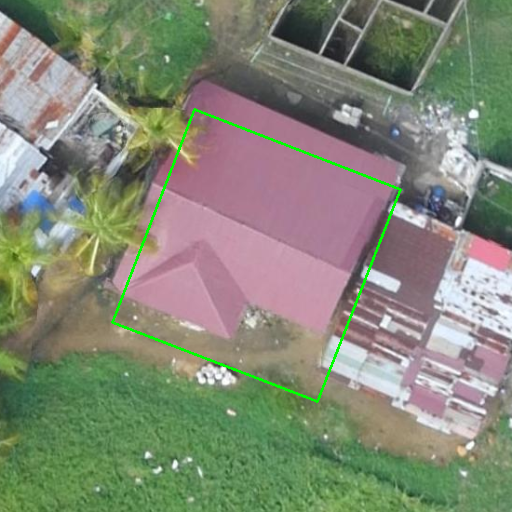
\includegraphics[width=\linewidth]{img/bld_0141916_clean.png}
    \caption{Original building footprint}
\end{subfigure}
\hfill
\begin{subfigure}{0.32\textwidth}
    \centering
    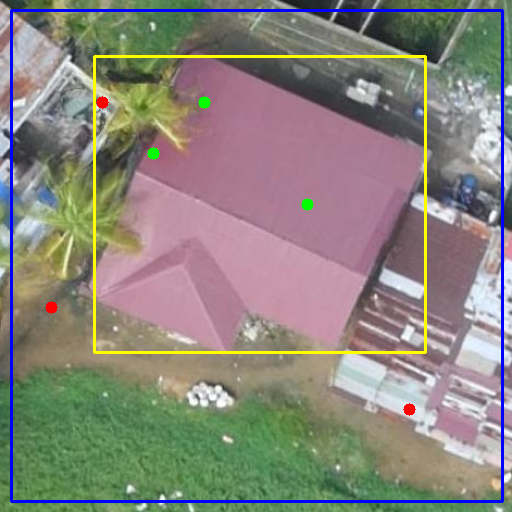
\includegraphics[width=\linewidth]{img/bld_0141916_sam_input.png}
    \caption{SAM prompt input}
\end{subfigure}
\hfill
\begin{subfigure}{0.32\textwidth}
    \centering
    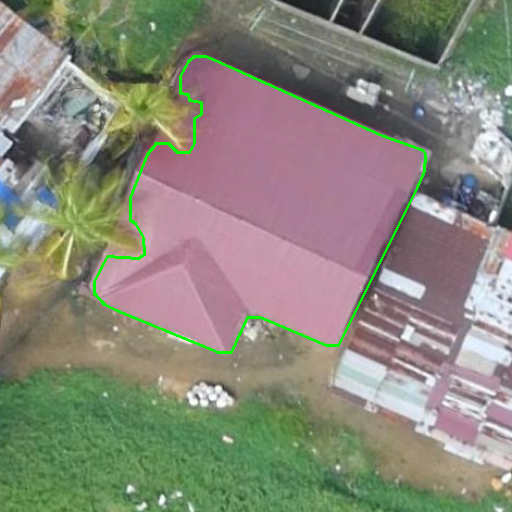
\includegraphics[width=\linewidth]{img/bld_0141916_sam.png}
    \caption{Refined segmentation result}
\end{subfigure}

\caption{FullHousePipeline refinement process. The existing building footprint provides spatial prompts that guide the segmentation model. Positive points, negative points, and a bounding box constrain the segmentation to refine the original footprint while preserving its approximate spatial extent. Own illustration.}
\label{fig:full_pipeline}

\end{figure}


In contrast, the \textit{PartialHousePipeline} addresses situations in which the original footprint captures only a subset of the visible building structure. In these cases, the polygon-derived bounding box may be too restrictive and would prevent the segmentation model from reconstructing the full building extent. Therefore, an additional detection step is introduced. Instead of restricting the model to the existing polygon, the text-prompted backend is used to identify all building structures within the image patch.

\begin{figure}[htb]
\centering

\begin{subfigure}[t]{0.24\textwidth}
    \vspace{0pt}
    \centering
    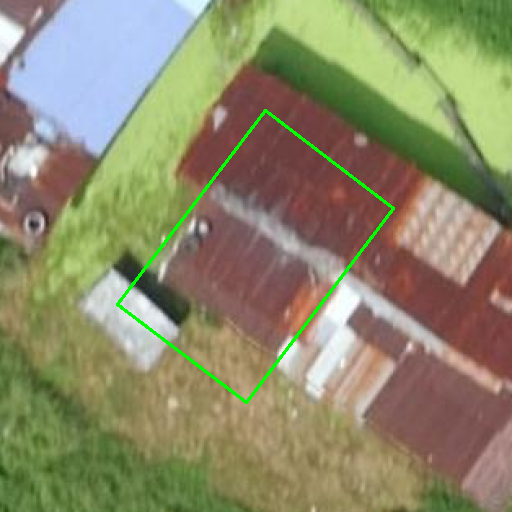
\includegraphics[width=\linewidth]{img/bld_1683655_clean.png}
    \caption{Incomplete footprint}
\end{subfigure}
\hfill
\begin{subfigure}[t]{0.24\textwidth}
    \vspace{0pt}
    \centering
    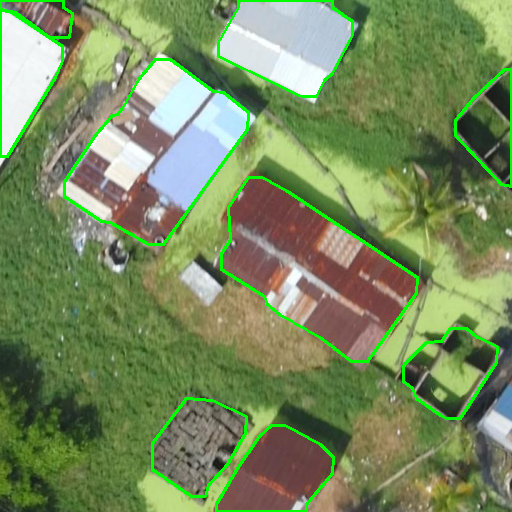
\includegraphics[width=\linewidth]{img/bld_1683655_detect_all_overlay.png}
    \caption{Text-prompted building discovery}
\end{subfigure}
\hfill
\begin{subfigure}[t]{0.24\textwidth}
    \vspace{0pt}
    \centering
    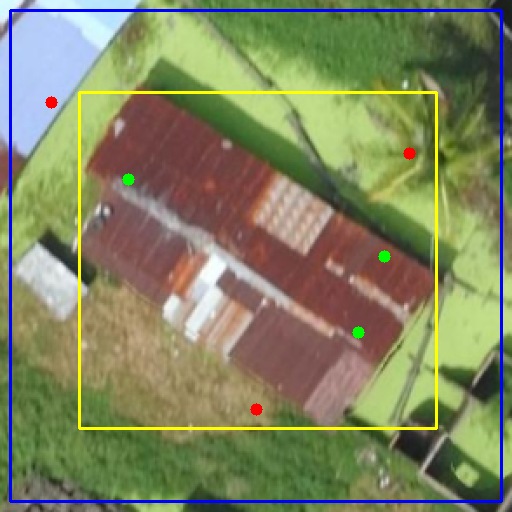
\includegraphics[width=\linewidth]{img/bld_1683655_sam_input.png}
    \caption{SAM prompt input}
\end{subfigure}
\hfill
\begin{subfigure}[t]{0.24\textwidth}
    \vspace{0pt}
    \centering
    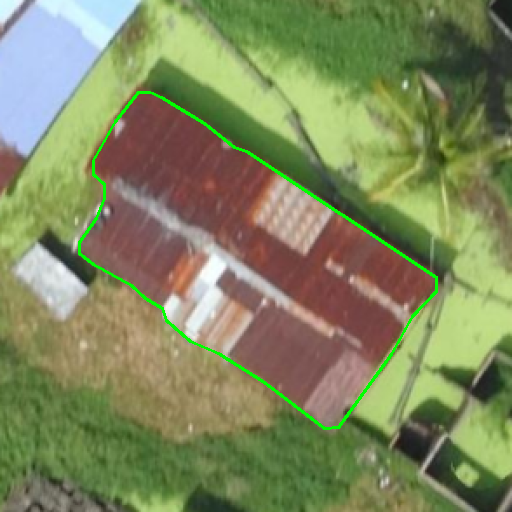
\includegraphics[width=\linewidth]{img/bld_1683655_sam.png}
    \caption{Refined building mask}
\end{subfigure}

\caption{PartialHousePipeline workflow. When the original footprint captures only part of the building, the spatial context is expanded and the segmentation model first performs a discovery step to identify the complete building structure before generating the final refined footprint. Own illustration.}

\label{fig:partial_pipeline_sam}

\end{figure}

For this discovery step, the implementation used the concept prompt ``roof''. The concept-prompted capability of SAM 3 allows the model to use semantic information in addition to spatial prompts.

This mechanism allows the model to detect complete building structures even when the initial footprint represents only a partial observation of the building. Once candidate roof regions have been identified, the candidate containing the original footprint centroid is selected; if no candidate contains the centroid, the nearest candidate centroid is used. The selected candidate is then passed to a local refinement crop where MLLM-generated positive and negative point prompts and the SAM-based visual-prompt backend produce the final refined building mask.
\subsection{Iterative Segmentation and Context Expansion}

Regardless of whether a building is routed through the \textit{FullHousePipeline} or the \textit{PartialHousePipeline}, the extracted patch ultimately passes through a common refinement stage in which the final building mask is generated using the SAM-based segmentation backend, as illustrated in Figure~\ref{fig:sam_stage}. In this stage, the multimodal large language model (MLLM) first generates spatial prompts in the form of positive and negative points. Together with an initial bounding box derived from the building footprint, these prompts serve as input for the visual segmentation backend. The segmentation process is performed iteratively. In the first iteration, a relatively large bounding box is used to ensure sufficient spatial context. After generating an initial mask, the bounding box is tightened to the extent of the predicted mask and the segmentation model is executed again to refine the segmentation. Where supported by the backend, segmentation logits from the previous iteration are passed to the next iteration. If the predicted polygon touches the boundary of the image patch, the system automatically extracts a larger patch to capture additional context. The refinement process was repeated for a maximum of three iterations or until no further context expansion was triggered.

\subsection{Polygon Extraction and Geometric Backprojection}

The segmentation model produces a binary mask in the \(512 \times 512\) patch coordinate system. This mask was converted into vector contours using OpenCV and subsequently into polygon geometries with Shapely. Small components and invalid geometries were removed or repaired before the polygon was transformed back into map coordinates. The inverse of the patch extraction transform was used to convert patch-pixel coordinates first to raster pixel coordinates and then to the raster CRS. The resulting polygon was stored in PostGIS together with the corresponding building identifier and run metadata.
\section{Post-processing}

The building polygons generated by the \textit{Segment Anything Model} (SAM) provide a strong initial representation of building footprints. However, due to the nature of image-based segmentation, the resulting geometries often contain inconsistencies that limit their direct usability for geospatial analysis. To address these issues, a structured post-processing pipeline is applied.

Three main types of geometric errors are observed:

\begin{itemize}
    \item \textbf{Fragmentation}: A single building may be represented by multiple adjacent or overlapping polygons. This is partly caused by inconsistencies in the source data and segmentation artifacts. These fragments are merged using geometric union operations combined with overlap-based grouping.
    \item \textbf{Irregular boundaries}: The segmentation process introduces small-scale noise along building edges, resulting in jagged or irregular raster-derived boundaries.
    \item \textbf{Tree occlusions}: Portions of building outlines are missing or distorted due to occlusion by vegetation. This leads to concave indentations or incomplete footprints and represents the most complex error type.
\end{itemize}

The post-processing pipeline addresses these issues step by step, combining geometric operations with simple assumptions about building shapes.

\subsection{Tree Occlusion}

Tree occlusions are handled by analyzing the spatial relationship between buildings and nearby trees. In the implementation, tree masks were generated with SAM 3 concept-prompted segmentation using the prompt ``tree'' and converted to polygon geometries before geometric repair. Let \(B\) be a building polygon and \(T\) the combined geometry of nearby trees.

First, a \textit{tree influence zone} is defined as a small area around the trees. This is done by slightly enlarging the tree geometry and subtracting a smaller inner buffer, where \(r_1\) and \(r_2\) denote the outer and inner tree-buffer radii, respectively:

\begin{equation}
Z_T = \operatorname{buffer}(T, r_1) \setminus \operatorname{buffer}(T, r_2).
\end{equation}

The tree influence zone \(Z_T\) represents the area where trees are likely to distort the building outline.

Next, possible occlusions are identified by intersecting this zone with the building boundary. The resulting candidate dent segments \(D_{\mathrm{cand}}\) are defined as:

\begin{equation}
D_{\mathrm{cand}} = \operatorname{boundary}(B) \cap Z_T.
\end{equation}

These candidate segments are split into smaller parts based on changes in direction. A segment is considered a candidate occlusion if it satisfies parameterized thresholds for distance to the tree boundary, minimum segment length, and deviation from a straight line.

Once such a dent is detected, the building shape is corrected. The idea is to reconstruct the missing part using the directions of the building edges before and after the dent.

Two simple cases are considered:

\begin{itemize}
    \item \textbf{Straight wall}: If both sides of the dent follow the same direction, the missing part is filled with a straight line.
    
    \item \textbf{Corner}: If the directions differ, the edges are extended until they meet, forming a new corner point.
\end{itemize}

To avoid unrealistic changes, the corrected polygon is only accepted if it remains similar to the original one. This is measured using the Intersection-over-Union (IoU), where \(B\) denotes the original polygon and \(B'\) the corrected polygon:

\begin{equation}
\operatorname{IoU}(B, B') =
\frac{\operatorname{area}(B \cap B')}{\operatorname{area}(B \cup B')}.
\end{equation}

The correction is applied only if this value is above a threshold.

This approach allows the reconstruction of building parts that were partially hidden by trees while preserving the overall shape of the building. The tree-occlusion component was custom-developed for this thesis. The main implementation parameters, including tree buffers, minimum overlap, and curvature thresholds, are listed in Appendix~\ref{app:core_parameters}.

\subsection{Polygon Regularization}
\label{sec:rectangularization}

After correcting tree occlusions, the building geometries are further refined to improve geometric regularity. The goal of this step is to reduce noise in the polygon boundaries while preserving the overall structure of the building.

Although this step is related to rectangularization, it does not enforce a single global orientation or force all buildings into idealized rectangular shapes.

As a baseline, the Python package \texttt{buildingregulariser} \citep{buildingregulariser} is used. However, this method was primarily developed for structured urban environments in highly planned regions, where buildings often follow consistent orientations and regular shapes. In such contexts, the algorithm applies strong assumptions, including a dominant global orientation and hard snapping of edges to predefined angles. These assumptions are less suitable for many regions in the Global South, where building layouts are often more irregular and do not follow a single dominant orientation. Applying a strict global alignment in such cases can lead to unrealistic distortions. To address this, a modified approach is used. Instead of deriving one global orientation for the full dataset, edge directions are analyzed separately for each polygon. The regularization first groups polygon edges into locally dominant direction clusters weighted by edge length and removes weak direction groups below a minimum weight ratio. The remaining dominant directions are ordered and constrained to orthogonal relationships. During angle enforcement, each sufficiently long edge is assigned to the nearest dominant direction group and then snapped fully to the nearest orthogonal target direction of that group if its deviation exceeds an adaptive tolerance. Very short edges are protected from this snapping step, and shorter retained edges use a larger tolerance. This makes the correction less intrusive for small boundary details while still reducing jagged mask-derived artifacts along the main building edges. After angle enforcement, the polygon is reconstructed and checked for geometric validity.

\section{Evaluation Strategy}
\label{sec:evaluation_strategy}

The evaluation approach is based on a manual assessment of building footprints across several regions in the Global South. The main objective is to determine whether the post-processed geometries produced by the pipeline improve upon the original input polygons. For each building, different aspects of geometric quality are examined, rather than relying on a single metric. The manual evaluation was based on visual agreement with the selected imagery rather than on independent cadastral ground truth.

To make the evaluation process efficient, a simple annotation tool was developed that allows quick navigation through the dataset and fast input of labels. The interface displayed the original polygon, the SAM-derived intermediate geometry, and the final post-processed geometry against the same imagery context (Figure~\ref{fig:evaluation_tool}). Ambiguous cases were rated conservatively according to the visible agreement between geometry and image evidence.

All manual ratings were assigned by the author using the same annotation interface and evaluation criteria. No independent second annotator was available; therefore, the labels should be interpreted as expert visual assessment rather than inter-annotator validated ground truth, and no inter-annotator agreement could be calculated.

In addition to the overall quality assessment, specific error types are recorded for both the original and the processed geometries. This enables an analysis of the dominant error sources before and after the pipeline. Furthermore, the manually assigned labels can be compared with the error descriptions generated by the multimodal model, allowing an assessment of how well the automated reasoning aligns with human evaluation.
\begin{figure}[htb]
	\centering  
	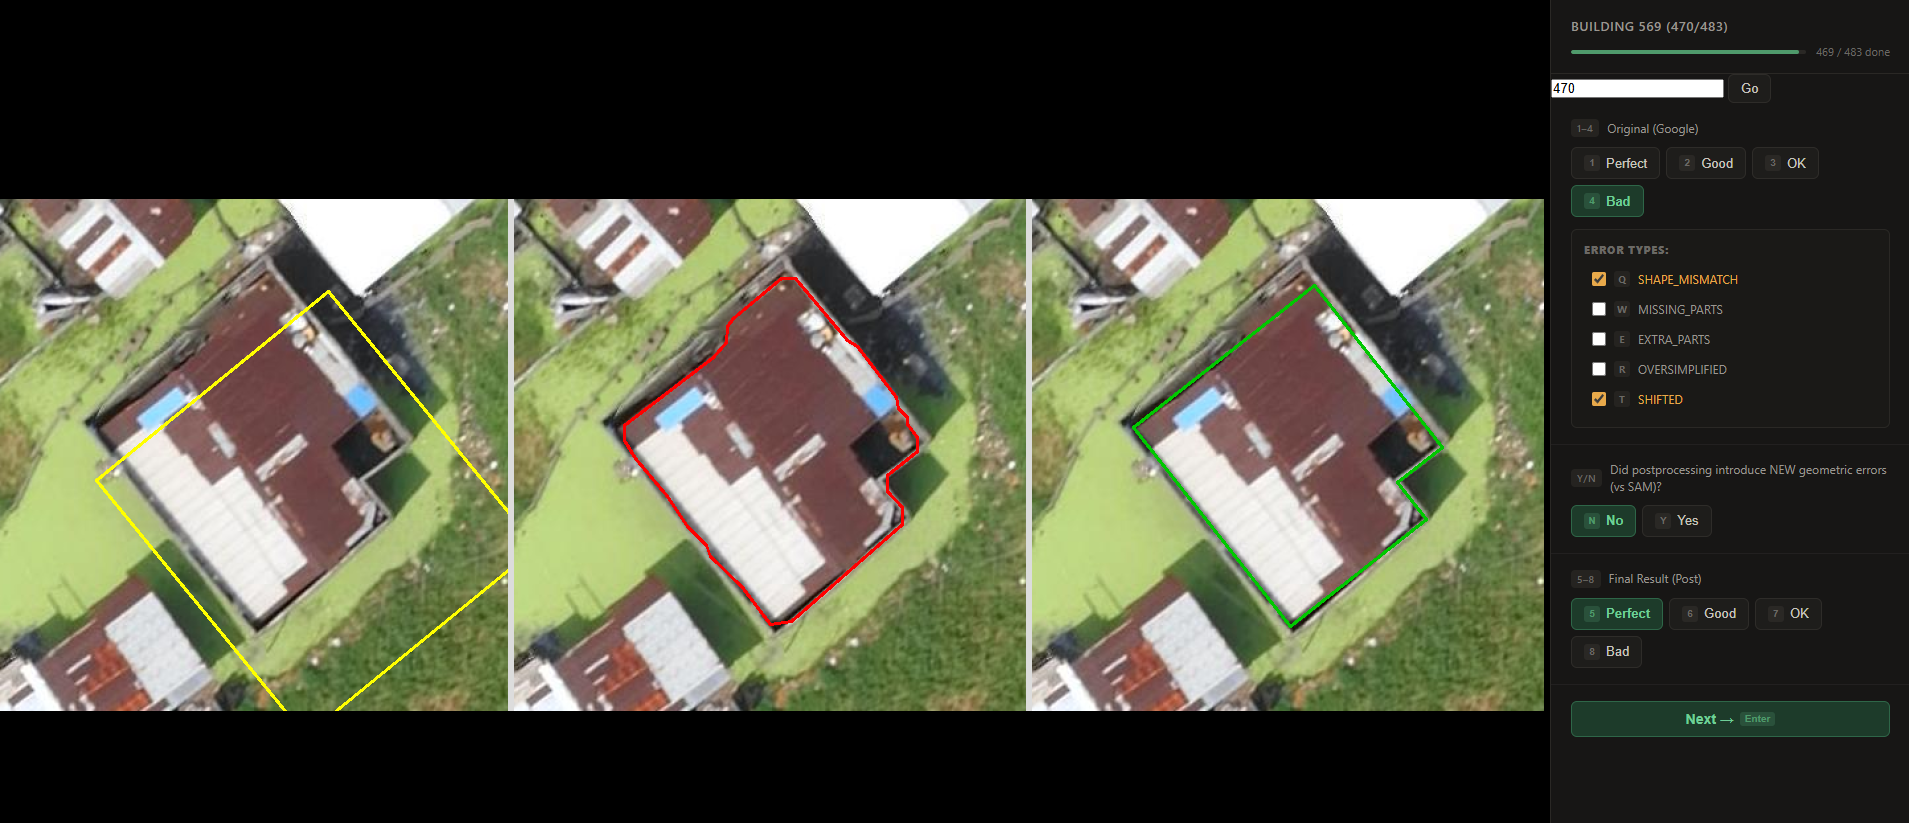
\includegraphics[scale=0.5]{Franzelin_Master/img/evaluation_tool.png}
	\caption{Annotation interface used for manual evaluation of original, SAM-derived, and post-processed building geometries. Own illustration.}
	\label{fig:evaluation_tool}
\end{figure}
\subsection{Evaluation Criteria and Error Taxonomy}
\label{sec:evaluation_criteria_error_taxonomy}

The geometric quality of building footprints is assessed using an ordinal rating scheme with four categories:

\begin{itemize}
    \item \textbf{Perfect:} The geometry closely matches the visible building outline without relevant visible errors.
    \item \textbf{Good:} Minor deviations are present, but the overall structure is correct.
    \item \textbf{OK:} Noticeable errors exist, though the building remains recognizable.
    \item \textbf{Bad:} The geometry is severely inaccurate or does not represent the building.
\end{itemize}

For the improvement analysis, the ordinal classes were ordered as \textit{Bad} < \textit{OK} < \textit{Good} < \textit{Perfect}. A post-processed polygon was counted as improved if its final rating was higher than the original rating, unchanged if it remained in the same class, and degraded if it received a lower rating.

In addition to the overall rating, multiple error categories can be assigned to each building:

\begin{itemize}
    \item \texttt{SHIFTED}: Correct shape but incorrect spatial position.
    \item \texttt{SHAPE\_MISMATCH}: Geometry does not match the visible building form.
    \item \texttt{MISSING\_PARTS}: Parts of the building are not captured.
    \item \texttt{EXTRA\_PARTS}: Geometry includes non-building areas.
    \item \texttt{OVERSIMPLIFIED}: Shape lacks geometric detail.
\end{itemize}

Additionally, it is recorded whether post-processing introduces new errors:

\begin{itemize}
    \item \textbf{No:} No additional errors introduced.
    \item \textbf{Yes:} New geometric errors introduced during post-processing.
\end{itemize}

\subsection{Reference-based Switzerland Test}
\label{sec:switzerland_reference_test}

In addition to the main evaluation in the five Global South study areas, a small reference-based test was carried out in Switzerland. This test was not used as the primary evaluation of the proposed workflow, because the overall research focus of this thesis is on regions without reliable reference building datasets. Instead, it served as an additional plausibility check in an area where authoritative building geometries are available.

For this test, building polygons from the Microsoft Global ML Building Footprints dataset \citep{microsoft_globalmlbuildingfootprints} were selected in a SWISSIMAGE scene \citep{swisstopo_swissimage} and processed with the same building extraction and regularization workflow. The resulting regularized building polygons were then compared against Swiss TLM building geometries from the Swiss topographic landscape model swissTLM3D, which was used as the authoritative reference dataset \citep{swisstopo_swisstlm3d}. The evaluation was implemented in a separate ArcPy script and performed in the Swiss coordinate reference system CH1903+ / LV95 (EPSG:2056), so that all area and distance calculations were carried out in meters.

Because the regularization run for the Switzerland scene was interrupted, the evaluation was restricted to the subset of Microsoft buildings for which a corresponding regularized output was available. To reconstruct this processed subset, available regularized outputs were matched back to the Microsoft source polygons using a 1\,m spatial buffer. The corresponding TLM reference buildings were then selected around the processed Microsoft subset, also using a 1\,m buffer. This ensured that both the original Microsoft polygons and the regularized polygons were evaluated against the same reference subset.

Candidate-reference pairs were generated from polygon intersections and then matched greedily in descending IoU order, so that each candidate polygon and each TLM reference polygon could be used at most once. The evaluation was repeated for IoU thresholds of 0.10, 0.25 and 0.50. For each threshold, true positives, false positives and false negatives were counted, and precision, recall and F1-score were calculated. The same procedure was applied once to the regularized output and once to the corresponding Microsoft source polygons, allowing a direct comparison between the input footprints and the newly generated regularized result.

\subsection{Evaluation of Semantic Error Descriptions}
\label{sec:evaluation_semantic_error_descriptions}

As part of the workflow, semantic error descriptions were generated for each extracted building patch. The generation process consisted of multiple stages. First, a dedicated prompt determined whether the polygon was shifted relative to the visible building footprint. Subsequently, a second prompt was instructed to ignore positional displacement and instead identify additional geometric error categories. The prompt explicitly specified the semantic categories and provided instructions explaining when each category should be assigned.

In addition to the structured category-based approach, an unrestricted free-text prompt was investigated. This prompt generated short human-readable explanations describing the mismatch between the original polygon and the visible building structure in the aerial image.

The free-text descriptions cannot be directly compared to manually assigned semantic labels because they consist of unconstrained natural language. Therefore, a rule-based text analysis was implemented to map recurring words and short phrase patterns back to the semantic taxonomy used during manual evaluation.

The analysis was performed only for buildings for which both manual reference labels and Multi-modal LLM Quality Assessment (MLQA)-generated semantic descriptions were available. Placeholder outputs such as \textit{No building detected} and parsing-error messages were excluded from the analysis.

For each description, the generated sentence was converted to lower case and searched for predefined keywords and phrase patterns. If one or multiple patterns associated with a semantic category were identified, the corresponding category was assigned to the sentence. Multiple semantic categories could therefore be extracted from a single generated description.

\begin{table}[htb]
\centering
\caption{Keyword and phrase mapping used to extract semantic error categories from MLQA-generated free-text descriptions.}
\label{tab:semantic_sentence_keyword_mapping}
\begin{tabular}{p{0.28\linewidth}p{0.62\linewidth}}
\hline
\textbf{Extracted category} & \textbf{Indicative words and phrases} \\
\hline

\texttt{SHIFTED} &
shifted, shift, offset, misaligned, misalignment, displaced, not aligned, away from \\

\texttt{SHAPE\_MISMATCH} &
shape, form, wrong, incorrect, mismatch, does not match, not matching, not following, deviates, distorted, irregular \\

\texttt{OVERSIMPLIFIED} &
oversimplified, oversimplification, too simplified, over simplified, lacks detail, low detail, too simple, generalized \\

\texttt{MISSING\_PARTS} &
missing, omitted, incomplete, not fully cover, not fully enclose, not fully capture, does not fully cover, cut off, uncovered \\

\texttt{EXTRA\_PARTS} &
extra, includes, non-building, surrounding area, surrounding ground, vegetation, beyond, extending into, outside the building, too large, over-extends \\

\hline
\end{tabular}
\end{table}

In addition to the rule-based text analysis, a small manual qualitative evaluation of the generated sentences was carried out. A separate annotation interface was created for this purpose. The interface displayed the aerial image patch with the original polygon overlay and the corresponding MLQA-generated error description. The evaluator assigned one of four sentence-quality labels: \textit{Correct}, \textit{Partly correct}, \textit{Too vague}, or \textit{Wrong}. Initially, 50 examples per study area were exported for this evaluation. However, while reviewing the generated descriptions it became apparent that the model repeatedly produced very similar sentence structures and reused the same terms, especially references to missing and extra parts. Therefore, the qualitative evaluation was limited to approximately 100 sentences, as additional samples were unlikely to provide substantially new insight into the linguistic behavior of the model.

Moreover, to evaluate whether the MLLM-generated spatial prompts were consistent with successful building refinements, an additional point-in-polygon analysis was performed. The analysis was restricted to buildings that were manually rated as \textit{perfect} after processing, because these geometries represent the most reliable available approximation of the visible roof outline. Only full-house cases were included, since the secondary crop transformations required to reconstruct point coordinates for partial-house cases were not stored. The results should therefore not be generalized to the harder partial-house branch. For each analyzable building, the generated positive and negative prompt points were transformed back into map coordinates and tested against the corresponding final polygon.

\subsection{Building-to-Surrounding Contrast Analysis}
\label{sec:building_surrounding_contrast}

An additional image-based analysis was carried out to compare the visual contrast between buildings and their immediate surroundings in the five study areas. This analysis was included because low roof-ground contrast was expected to influence both the MLLM visibility decision and the SAM-based segmentation step.

For the automatic analysis, all post-processed buildings that received the manual quality label \textit{perfect} were selected. For each selected building, the final post-processed polygon was transformed into patch pixel coordinates and rasterized as the building mask. A local surrounding mask was then created by buffering the polygon outward by 48 pixels and subtracting an inner 4-pixel gap around the building boundary. The gap reduces direct edge effects caused by antialiasing, shadows, or small boundary misalignments. Pixels covered by neighboring building polygons were excluded from the surrounding mask so that the background measurement represented local ground context as far as possible. If the cleaned ring contained too few pixels, the remaining non-building pixels in the patch were used as a fallback background mask.

For each building, the mean brightness inside the building mask and inside the surrounding ring was calculated. The RGB values were first converted to linearized relative luminance so that the brightness comparison was not based directly on gamma-encoded image values. Denoting these luminance values by $Y_{\mathrm{building}}$ and $Y_{\mathrm{surrounding}}$, respectively, the final contrast value (C) used in the results is the absolute Weber contrast, a relative luminance-difference measure between a target and its background \citep{PelliBex2013}:


\begin{equation}
C = \left|
\frac{Y_{\mathrm{building}} - Y_{\mathrm{surrounding}}}
{Y_{\mathrm{surrounding}}}
\right|.
\end{equation}

This value describes how strongly the building differs in brightness from its local background, independent of whether the roof is brighter or darker than the surroundings. In addition, a simple texture-difference value was calculated using the same building and ring masks. The texture value combines three local image descriptors: Sobel gradient magnitude, absolute Laplacian response, and local standard deviation in a \(9 \times 9\) window. The Euclidean distance between the building texture descriptor and the surrounding texture descriptor was used as the final texture-difference value. It should be interpreted as a compact indicator of whether roof and background differ in edge density and local image variation.

The contrast and texture measures are used here as descriptive image statistics rather than as independent validation metrics.

\section{Implementation Details}

While the previous sections describe the methodological design of the workflow, this section summarizes the practical implementation choices required to execute the pipeline reproducibly. The implementation consists of a local Python-based geospatial processing environment, a PostgreSQL/PostGIS database for persistent spatial data management, and a remote GPU inference service for the multimodal model.

The processing code is organized as a modular Python project. The main entry point is \texttt{src/main.py}. Raster patch extraction is implemented in \texttt{patches/}, multimodal quality assessment in \texttt{mlqa/}, refinement logic in \texttt{pipelines/}, SAM-based segmentation in \texttt{sam/}, database operations in \texttt{db/}, and geometric post-processing in \texttt{postprocess/}. This structure separates processing responsibilities and allows individual components, such as the MLLM or segmentation backend, to be exchanged without modifying the complete workflow.

In addition to the evaluated per-building workflow, the code repository contains a tiled global-discovery extension that applies SAM 3 concept-prompted segmentation with the prompt ``roof'' to search for additional roof candidates. This component was treated as an exploratory extension and was not central to the reported quantitative evaluation.

Dependency management was handled using \texttt{uv}, a high-performance Python package and project manager \citep{uv_docs}. The main pipeline was executed in a project-specific Python 3.11 environment containing geospatial, computer vision, database, and model inference dependencies. Important libraries include \texttt{geopandas}, \texttt{rasterio}, \texttt{shapely}, \texttt{pyproj}, \texttt{opencv-python}, \texttt{torch}, \texttt{sqlalchemy}, \texttt{psycopg2}, and the OpenAI Python client. A separate virtual environment was used for the post-processing module, where the \texttt{buildingregulariser} package was linked as a locally editable dependency.

Persistent storage was implemented using PostgreSQL together with the PostGIS spatial extension, providing spatial indexing and geometry operations required for large-scale vector processing. Database access was configured through the environment variable \texttt{PG\_CONN}. The import scripts create the schema \texttt{src}, enable PostGIS, define required spatial tables, and generate spatial indexes.

The multimodal model was deployed separately from the local geospatial pipeline. Qwen3-VL-8B-Instruct was served on a RunPod GPU instance using \texttt{vLLM}, a high-throughput LLM serving framework designed for efficient inference and memory management through PagedAttention \citep{kwon2023pagedattention}. The model server exposes an OpenAI-compatible API, allowing the local Python code to communicate with the remote model through the standard OpenAI client interface. The RunPod instance is referenced through the environment variable \texttt{RUNPOD\_ID}, from which the endpoint URL is constructed. In this setup, the OpenAI client is used only as an API wrapper; the actual inference is performed by the self-hosted vLLM server.

Each pipeline run is assigned a unique \texttt{RUN\_ID}, which is written together with all detected geometries. This enables separation and comparison of different experimental runs within the database.
